\documentclass[tikz]{standalone}
\usepackage{ctex}
\usepackage{tikz}
\usepackage{pgfplots}
\pgfplotsset{compat=1.18}   % 使用较新版本语法
\usetikzlibrary{positioning, arrows.meta, intersections, calc, fit, backgrounds}
\usepgfplotslibrary{fillbetween}  % 用于填充区域

\begin{document}
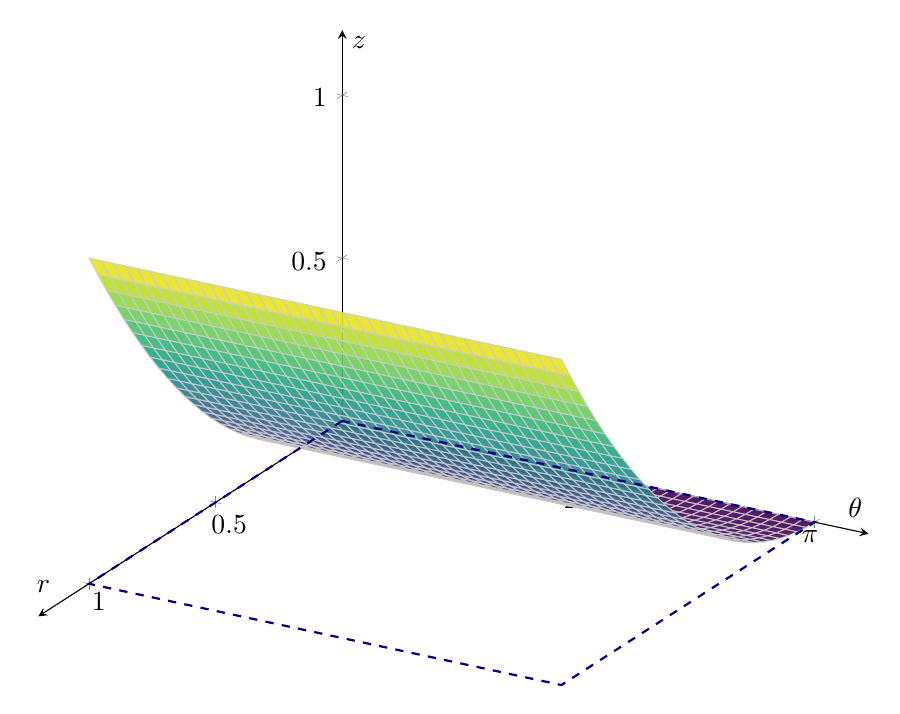
\begin{tikzpicture}
    \begin{axis}[
            view={120}{30},                     % 视角
            axis lines=center,
            xlabel={$r$}, ylabel={$\theta$}, zlabel={$z$},
            xtick={0,0.5,1},
            ytick={0,1.5708,3.14159},
            yticklabels={$0$, $\frac{\pi}{2}$, $\pi$},
            ztick={0,0.5,1},
            xmin=0, xmax=1.2,
            ymin=0, ymax=3.5,
            zmin=0, zmax=1.2,
            colormap/viridis,
            samples=30,
            width=\textwidth,   % 宽度设置为 0.8 倍版心宽
            samples y=40,
            clip=false
        ]
        % 曲面 z = r^2 定义在矩形区域 r ∈ [0,1], θ ∈ [0,π]
        \addplot3[
            surf,
            domain=0:1,
            domain y=0:pi,
            opacity=0.85,
            faceted color=black!20,
            fill opacity=0.9
        ] ({x}, {y}, {x^2});
        % 绘制底部矩形区域的边界（积分区域）
        \draw[thick, dashed, blue!50!black]
        (axis cs:0,0,0) -- (axis cs:1,0,0) --
        (axis cs:1,pi,0) -- (axis cs:0,pi,0) -- cycle;
    \end{axis}
\end{tikzpicture}
\end{document}